% !TEX encoding = UTF-8 Unicode
% !TEX program  = pdflatex
%
% Smart-Traffic-MARL — Báo cáo bài tập lớn môn Machine Learning
% Template: IEEE Conference (two-column)
% Ngôn ngữ: Tiếng Việt (babel + inputenc)
%

\documentclass[conference]{IEEEtran}

% ── Encoding & Vietnamese ─────────────────────────────────────────────────────
\usepackage[utf8]{inputenc}
\usepackage[vietnamese]{babel}

% ── Packages ──────────────────────────────────────────────────────────────────
\usepackage{amsmath,amssymb,amsfonts}
\usepackage{graphicx}
\usepackage{booktabs}
\usepackage{multirow}
\usepackage{hyperref}
\usepackage{algorithm}
\usepackage{algorithmic}
\usepackage{xcolor}
\usepackage{subcaption}
\usepackage{url}
\usepackage{enumitem}

\hypersetup{
    colorlinks=true,
    linkcolor=blue,
    citecolor=blue,
    urlcolor=blue,
}

% ── Macros ────────────────────────────────────────────────────────────────────
\newcommand{\eg}{\textit{e.g.}}
\newcommand{\ie}{\textit{i.e.}}
\newcommand{\etc}{\textit{etc.}}

% ══════════════════════════════════════════════════════════════════════════════
\begin{document}

\title{\resizebox{\linewidth}{!}{GAT-MARL: Điều phối mạng lưới đèn giao thông đô thị} \\ 
bằng Multi-Agent Reinforcement Learning \\ 
và Graph Attention Network}

\author{
\IEEEauthorblockN{Đặng Quang Minh, Ngô Trọng Hiệp, Khổng Quang Huy}% <-this % stops a space
\\ Viện Trí tuệ nhân tạo \\
Trường Đại học Công nghệ -- Đại học Quốc gia Hà Nội \\
144 Xuân Thuỷ, Cầu Giấy, Hà Nội, Việt Nam \\
{\tt\small\{24022397, 24022325, 24022355\}@vnu.edu.vn} \\ \\
% Nhóm 13 — Bài tập lớn môn Machine Learning, HK2 2025--2026
}

\maketitle

% ══════════════════════════════════════════════════════════════════════════════
%  ABSTRACT
% ══════════════════════════════════════════════════════════════════════════════
\begin{abstract}
Báo cáo này trình bày hệ thống GAT-MARL --- một phương pháp điều phối mạng lưới đèn giao thông đô thị dựa trên Multi-Agent Reinforcement Learning (MARL) kết hợp Graph Attention Network (GAT). Bài toán được mô hình hóa dưới dạng Dec-POMDP và kiểm chứng trên hai mạng lưới thực tế tại Hà Nội: Mỹ Đình (8 ngã tư) và khu vực Đại học Công nghệ --- UET (15 ngã tư). Kiến trúc đề xuất sử dụng parameter sharing toàn phần, reward function hybrid (waiting time + weighted pressure) với normalization, và phương pháp training parallel kiểu Ape-X với fixed-role epsilon workers. Thực nghiệm cho thấy GAT-MARL hội tụ nhanh hơn và đạt hiệu năng cao hơn so với Independent DQN và fixed-time baseline, đồng thời thể hiện khả năng chuyển giao kiến thức hiệu quả sang topology mới thông qua cơ chế 2-phase fine-tuning.
\end{abstract}

\begin{IEEEkeywords}
Điều khiển đèn giao thông, Multi-Agent Reinforcement Learning, Graph Attention Network, Deep Q-Network, SUMO
\end{IEEEkeywords}

% ══════════════════════════════════════════════════════════════════════════════
%  1. GIỚI THIỆU
% ══════════════════════════════════════════════════════════════════════════════
\section{Giới thiệu}

Tắc nghẽn giao thông đô thị là vấn đề nghiêm trọng tại các thành phố lớn ở Việt Nam, đặc biệt tại Hà Nội. Hệ thống đèn tín hiệu truyền thống hoạt động theo chu kỳ cố định, không phản ứng linh hoạt với lưu lượng xe thực tế, dẫn đến lãng phí thời gian chờ và ùn tắc cục bộ.

Reinforcement Learning (RL) đã được chứng minh là hướng tiếp cận hiệu quả cho bài toán adaptive traffic signal control (ATSC)~\cite{PressLight2019, CoLight2019, MPLight2020}. Tuy nhiên, các phương pháp Independent RL gặp hạn chế khi mỗi agent chỉ quan sát ngã tư của mình, thiếu khả năng phối hợp toàn mạng. CoLight~\cite{CoLight2019} đề xuất sử dụng Graph Attention Network~\cite{Velickovic2018} để cho phép các agent giao tiếp qua cơ chế attention, đạt kết quả vượt trội trên nhiều bộ dữ liệu.

Báo cáo trình bày hệ thống GAT-MARL được xây dựng và kiểm chứng trên hai mạng lưới giao thông thực tế tại Hà Nội, với các đóng góp chính:

\begin{itemize}[leftmargin=*]
    \item Thiết kế reward function hybrid kết hợp waiting time (70\%) và weighted pressure (30\%) với normalization về $[0, 1]$ trước khi scale, đảm bảo hai thành phần có cùng đơn vị.
    \item Hệ thống parallel training kiểu Ape-X~\cite{ApeX2018} với fixed-role epsilon workers, tạo dữ liệu đa dạng từ explorer đến near-greedy.
    \item Dynamic lane detection theo topology thực tế --- hỗ trợ đường arterial 3 làn và secondary 2 làn trên cùng một mạng lưới.
    \item Mô phỏng sự cố giao thông (obstacle injection) trong quá trình training để tăng robustness.
    \item Dashboard real-time theo dõi và so sánh 3 phương pháp song song: Fixed-time, IDQN, và GAT-MARL.
\end{itemize}

% ══════════════════════════════════════════════════════════════════════════════
%  2. CƠ SỞ LÝ THUYẾT
% ══════════════════════════════════════════════════════════════════════════════
\section{Cơ sở lý thuyết}

\subsection{Multi-Agent Reinforcement Learning}

Bài toán điều khiển đèn giao thông với $N$ ngã tư được mô hình hóa dưới dạng Decentralized Partially Observable Markov Decision Process (Dec-POMDP), trong đó mỗi ngã tư là một agent quyết định pha đèn dựa trên quan sát cục bộ.

Thách thức cơ bản của MARL là \textbf{non-stationarity}: khi các agent đồng thời cập nhật policy, môi trường trở nên non-stationary từ góc nhìn của từng agent đơn lẻ --- điều kiện Markov bị vi phạm vì transition probability phụ thuộc vào policy của agents khác, không chỉ state hiện tại. Đây là lý do Independent Q-Learning không có đảm bảo hội tụ trong setting đa agent.

Hai chiến lược MARL phổ biến:
\begin{itemize}[leftmargin=*]
    \item \textbf{Independent learning}: mỗi agent học riêng rẽ, coi các agent khác là một phần của môi trường. Đơn giản nhưng vi phạm giả thiết Markov do non-stationarity.
    \item \textbf{Networked/Cooperative learning}: các agent chia sẻ thông tin qua cơ chế communication, giảm non-stationarity bằng cách làm cho joint policy trở thành một phần của quan sát. CoLight~\cite{CoLight2019} là đại diện tiêu biểu với GAT làm communication layer. Trong hệ thống này, GAT cho phép mỗi agent quan sát trạng thái của các neighbors, kết hợp shared reward để gradient update của từng agent phản ánh kết quả toàn mạng --- hai cơ chế này phối hợp giảm thiểu ảnh hưởng của non-stationarity.
\end{itemize}

\subsection{Deep Q-Network và Double DQN}

DQN~\cite{Mnih2015} xấp xỉ hàm Q bằng mạng neural sâu, sử dụng experience replay và target network để ổn định training. Tuy nhiên, DQN có xu hướng overestimate Q-values do sử dụng cùng một mạng để chọn và đánh giá action.

Double DQN~\cite{vanHasselt2016} khắc phục bằng cách tách biệt hai bước: mạng online chọn action tốt nhất, mạng target đánh giá giá trị:
\begin{equation}
    y_t = r_t + \gamma \, Q_{\theta^{-}}\!\left(s_{t+1},\, \arg\max_{a} Q_\theta(s_{t+1}, a)\right)
    \label{eq:ddqn}
\end{equation}
trong đó $\theta$ là tham số mạng online, $\theta^{-}$ là tham số target network.

\subsection{Graph Attention Network}

GAT~\cite{Velickovic2018} áp dụng cơ chế self-attention lên dữ liệu đồ thị, cho phép mỗi node tự động học trọng số attention với các neighbors. Đặt $e_{ij} = \mathbf{a}^T [\mathbf{W}\mathbf{h}_i \| \mathbf{W}\mathbf{h}_j]$, hệ số attention được tính:
\begin{equation}
    \alpha_{ij} = \frac{\exp(\text{LReLU}(e_{ij}))}{\displaystyle\sum_{k \in \mathcal{N}_i} \exp(\text{LReLU}(e_{ik}))}
    \label{eq:gat_attn}
\end{equation}
trong đó $\text{LReLU}(\cdot)$ là LeakyReLU. Với multi-head attention ($K$ heads), output được average:
\begin{equation}
    \mathbf{h}'_i = \sigma\!\left(\frac{1}{K} \sum_{k=1}^{K} \sum_{j \in \mathcal{N}_i} \alpha_{ij}^k \mathbf{W}^k \mathbf{h}_j\right)
    \label{eq:gat_multihead}
\end{equation}

Đặc điểm quan trọng của GAT là không yêu cầu trọng số edge được định nghĩa trước, phù hợp với mạng giao thông nơi mức độ ảnh hưởng giữa các ngã tư thay đổi theo lưu lượng và thời điểm trong ngày.

\subsection{Max Pressure và PressLight}

Max Pressure~\cite{PressLight2019} định nghĩa ``áp suất'' tại ngã tư $i$ dựa trên chênh lệch queue giữa incoming và outgoing edges. PressLight~\cite{PressLight2019} là framework RL đầu tiên kết hợp lý thuyết Max Pressure vào thiết kế reward, chứng minh tính tối ưu lý thuyết khi throughput hội tụ.

MPLight~\cite{MPLight2020} mở rộng PressLight với parameter sharing, cho phép scale lên hàng nghìn ngã tư. Hệ thống kế thừa cả hai ý tưởng: pressure làm regularizer trong reward, parameter sharing cho toàn bộ agents.

% ══════════════════════════════════════════════════════════════════════════════
%  3. MÔ TẢ HỆ THỐNG
% ══════════════════════════════════════════════════════════════════════════════
\section{Mô tả hệ thống}

\subsection{Môi trường mô phỏng SUMO}

Hệ thống sử dụng SUMO (Simulation of Urban Mobility)~\cite{SUMO2018} --- trình mô phỏng giao thông vi mô chuẩn công nghiệp, giao tiếp qua TraCI API.

\textbf{Bản đồ Mỹ Đình}: 8 ngã tư thực tế (N01--N08), mô phỏng khu vực giao giữa các trục: Hồ Tùng Mậu (arterial ngang), Lê Đức Thọ và Phạm Hùng (arterial dọc), Nguyễn Cơ Thạch (secondary dọc trái), Hàm Nghi, Nguyễn Hoàng, và Trần Hữu Dực (secondary ngang) (Hình~\ref{fig:topology}).

\begin{figure}[!t]
    \centering
    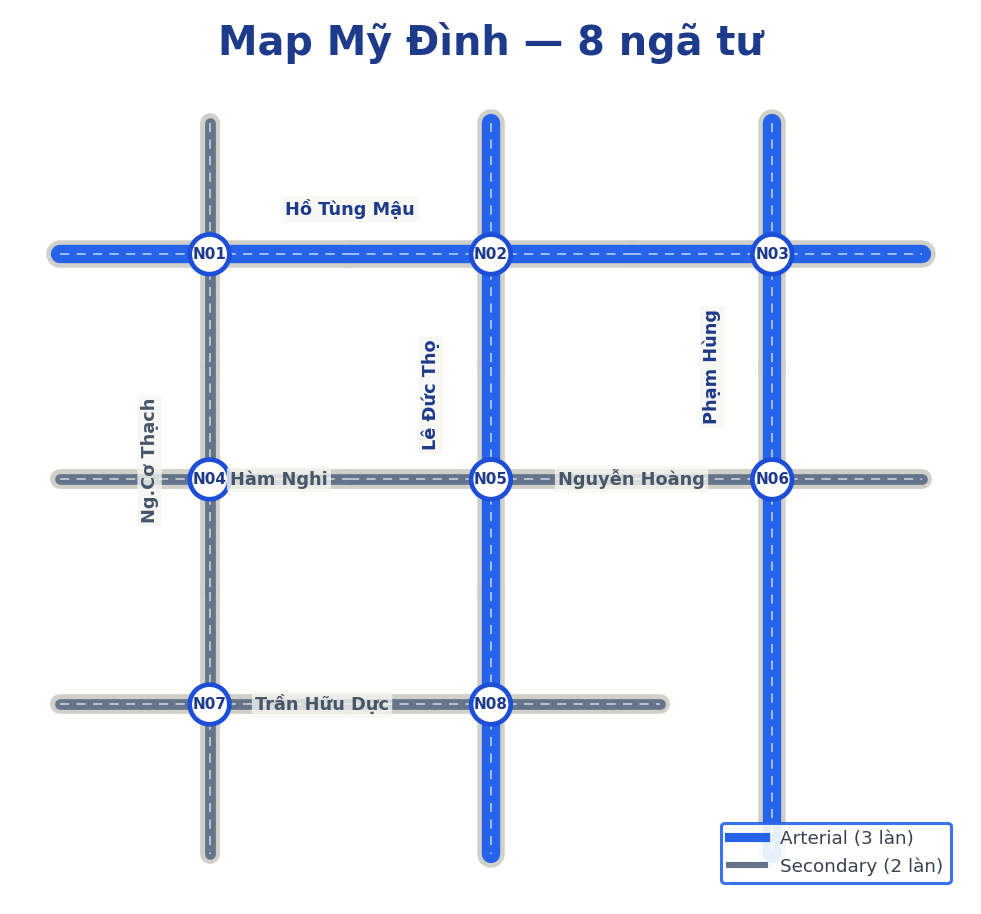
\includegraphics[width=\linewidth]{imgs/map_mydinh.png}
    \caption{Topology mạng lưới giao thông khu vực Mỹ Đình (8 ngã tư).}
    \label{fig:topology}
\end{figure}

\textbf{Cấu hình mô phỏng}: mỗi episode kéo dài 1800 giây (30 phút), decision step $\Delta t = 5$s (tổng 360 bước/episode). Mỗi episode lấy ngẫu nhiên một trong ba kịch bản lưu lượng: \texttt{peak\_morning} (35\%), \texttt{peak\_evening} (35\%), và \texttt{night} (30\%), phản ánh phân bố lưu lượng thực tế trong ngày.

\subsection{State Space}

State vector cho mỗi ngã tư $i$ có chiều $d_s$ được tính \textit{tự động} theo topology:
\begin{equation}
    d_s = 2 \times L_{\max} + N_{\text{phase}} + 1
    \label{eq:state_dim}
\end{equation}
trong đó $L_{\max} = \max_i \sum_{e \in \mathcal{E}_i^{\text{in}}} n_e$ là \textbf{tổng số lanes trên tất cả incoming edges} của ngã tư có nhiều lanes nhất (tính bằng cách cộng dồn $n_e$ của mọi incoming edge $e$, không phải max từng edge riêng lẻ), $N_{\text{phase}} = 4$ (one-hot), và 1 chiều cho time-since-change. Trên map Mỹ Đình, $L_{\max} = 8$ cho $d_s = 2 \times 8 + 4 + 1 = 21$.

Cụ thể, state vector gồm:
\begin{itemize}[leftmargin=*]
    \item \textbf{Density per lane} ($L_{\max}$ chiều): occupancy normalize $[0, 1]$ từ E2 detector.
    \item \textbf{Queue per lane} ($L_{\max}$ chiều): halting vehicle count normalize bởi $\text{MAX\_QUEUE} = 20$.
    \item \textbf{Phase one-hot} (4 chiều): NS\_green, NS\_yellow, EW\_green, EW\_yellow.
    \item \textbf{Time since change} (1 chiều): normalize bởi 120 giây.
\end{itemize}

Hàm \texttt{get\_edge\_lanes()} trả về số lane thực tế của từng edge (3 làn cho arterial, 2 làn cho secondary), đảm bảo state vector phản ánh đúng topology. Các ngã tư có ít lanes hơn $L_{\max}$ được pad~0.

\subsection{Action Space}

Action space nhị phân cho mỗi agent: $a_i \in \{0, 1\}$
\begin{itemize}[leftmargin=*]
    \item $a = 0$: giữ nguyên pha hiện tại (keep).
    \item $a = 1$: chuyển sang pha tiếp theo (switch) --- trigger yellow phase trước khi chuyển green.
\end{itemize}

Constraint min-green ($\geq 20$s) và yellow cố định ($3$s) được enforce ở tầng environment, không phải model --- đảm bảo tính hợp lệ mà agent không cần học.

\subsection{Reward Function}
\label{sec:reward}

Reward function được thiết kế dạng hybrid, kết hợp hai tín hiệu, cả hai đều được \textbf{normalize về $[0, 1]$} trước khi kết hợp:
\begin{equation}
    r_i = -\left(\alpha \cdot \hat{w}_i + \beta \cdot \hat{p}_i\right) \times S
    \label{eq:reward}
\end{equation}
trong đó:
\begin{itemize}[leftmargin=*]
    \item $\hat{w}_i = \min\!\left(\bar{w}_i,\, W_{\max}\right) / W_{\max}$ --- waiting time trung bình normalize, clip tại $W_{\max} = 120$s.
    \item $\hat{p}_i = \min\!\left(p_i,\, P_{\max}\right) / P_{\max}$ --- weighted pressure normalize, clip tại $P_{\max} = 5.0$.
    \item $\alpha = 0.7,\; \beta = 0.3$ --- waiting time chiếm 70\% (primary signal, sát tiêu chí HCM~7th Edition); pressure chiếm 30\% (regularizer, phản ánh mức độ mất cân bằng queue).
    \item $S = 5.0$ --- reward scale, đảm bảo gradient đủ lớn.
\end{itemize}

\textbf{Weighted pressure} tính có trọng số theo tầm quan trọng đường:
\begin{equation}
    p_i = \frac{\left|\sum_{e \in \mathcal{E}_i^{\text{in}}} w_e \cdot q_e - \sum_{e \in \mathcal{E}_i^{\text{out}}} w_e \cdot q_e\right|}{|\mathcal{L}_i|}
    \label{eq:pressure}
\end{equation}
với $w_e = 2.0$ cho arterial (Hồ Tùng Mậu, Lê Đức Thọ, Phạm Hùng trên map Mỹ Đình; Hồ Tùng Mậu, Xuân Phương, Phạm Hùng trên map UET), $w_e = 1.0$ cho secondary.

\textbf{Teleport penalty}: khi xe kẹt quá 300s, SUMO teleport xe ra khỏi mạng. Penalty chia đều cho tất cả agents, cap tại 2.5:
\begin{equation}
    \text{penalty} = \min\!\left(\frac{0.5 \times n_{\text{teleport}}}{N_{\text{agents}}} \times S,\; 2.5\right)
\end{equation}

\textbf{Shared reward (GAT-MARL)}: để khuyến khích cooperative behavior trong quá trình \textit{training}, reward mỗi agent GAT được tính theo dạng hybrid: $r_i^{\text{train}} = 0.7 \cdot r_i + 0.3 \cdot \bar{r}$, trong đó $\bar{r} = \frac{1}{N}\sum_{j} r_j$ là mean reward toàn mạng. Thiết kế này giữ lại 70\% tín hiệu individual để Q-values không collapse về nhau (mỗi agent vẫn phân biệt được khi mình hoạt động tốt hay kém), đồng thời 30\% global mean thúc đẩy coordination. Cơ chế này chỉ áp dụng ở tầng \texttt{train\_parallel.py} (worker loop), không ảnh hưởng đến inference. IDQN giữ individual reward vì không có communication layer để leverage shared signal.

% ══════════════════════════════════════════════════════════════════════════════
%  4. KIẾN TRÚC MÔ HÌNH
% ══════════════════════════════════════════════════════════════════════════════
\section{Kiến trúc mô hình}

\subsection{GAT-MARL Network}

Kiến trúc theo hướng tiếp cận của CoLight~\cite{CoLight2019} với parameter sharing toàn phần theo MPLight~\cite{MPLight2020}, gồm 3 module dùng chung trọng số cho tất cả $N$ agents (Hình~\ref{fig:architecture}):

\begin{figure}[h]
    \centering
    \fbox{\parbox{0.9\linewidth}{\centering\vspace{1em}
    \small
    \texttt{obs\_i ($d_s$)} $\rightarrow$ \texttt{[LocalEncoder: MLP]} $\rightarrow$ $\mathbf{h}_i \in \mathbb{R}^{64}$\\[0.4em]
    $\mathbf{h}_1,\ldots,\mathbf{h}_N$ $\xrightarrow{\text{GATConv (4 heads)}}$ $\mathbf{h}'_i \in \mathbb{R}^{64}$\\[0.4em]
    $\mathbf{h}'_i$ $\rightarrow$ \texttt{[Q-head: MLP]} $\rightarrow$ $Q(s,\text{keep}),\; Q(s,\text{switch})$\\[0.6em]
    \textit{(Toàn bộ agents dùng chung 1 bộ trọng số)}
    \vspace{1em}}}
    \caption{Kiến trúc GAT-MARL. Tất cả agents dùng chung bộ trọng số --- GAT tự differentiate agent qua graph topology.}
    \label{fig:architecture}
\end{figure}

\textbf{1) Local Encoder} (Shared MLP): $\texttt{Linear}(d_s, 64) \to \texttt{ReLU} \to \texttt{Linear}(64, 64) \to \texttt{ReLU}$. Mã hóa observation thô thành hidden representation $\mathbf{h}_i \in \mathbb{R}^{64}$.

\textbf{2) GAT Communication Layer}: sử dụng \texttt{GATConv}~\cite{Velickovic2018} từ PyTorch Geometric~\cite{PyG2019} với 4 attention heads, \texttt{concat=False} (output giữ nguyên 64 chiều), \texttt{add\_self\_loops=True}, dropout $= 0.1$. Output $\mathbf{h}'_i$ chứa thông tin enriched từ neighbors.

\textit{Lưu ý về self-loop}: với \texttt{add\_self\_loops=True}, \texttt{GATConv} tự thêm $N$ self-loop edges vào \texttt{edge\_index} trước khi tính attention, do đó $\mathcal{N}_i$ trong công thức~\eqref{eq:gat_attn} bao gồm cả node $i$. Hệ quả kỹ thuật: \texttt{\_attention\_weights} sau forward có shape $(E + N,)$ thay vì $(E,)$. Khi chuyển về attention matrix $(N \times N)$, cần augment \texttt{edge\_index} tương ứng (xem \texttt{get\_attention\_matrix()} trong \texttt{gat\_marl.py}).

\textbf{3) Q-head} (Shared MLP): $\texttt{Linear}(64, 64) \to \texttt{ReLU} \to \texttt{Linear}(64, 2)$. Xuất Q-values cho 2 actions.

\textbf{Batched graph processing}: khi training, $B$ samples được ghép thành 1 batch graph lớn. Edge index được repeat với offset $b \times N$ cho mỗi sample $b$, tạo thành \texttt{(2, B$\times$E)} --- forward 1 lần qua GAT thay vì $B$ lần.

\subsection{Independent DQN (Baseline)}

IDQN có cùng Local Encoder và Q-head nhưng \textbf{không có GAT layer} --- mỗi agent forward độc lập. Vẫn dùng parameter sharing (1 network cho $N$ agents) và Double DQN. So sánh IDQN vs GAT-MARL cho thấy tác dụng của communication qua GAT.

\subsection{Fixed-time (Baseline)}

Chu kỳ cố định 30s green + 3s yellow, không có khả năng thích ứng. Được dùng làm baseline tham chiếu (lower-bound) trong so sánh hiệu năng.

% ══════════════════════════════════════════════════════════════════════════════
%  5. PHƯƠNG PHÁP TRAINING
% ══════════════════════════════════════════════════════════════════════════════
\section{Phương pháp training}

\subsection{Parallel Training --- Ape-X Style}

Hệ thống training parallel (Hình~\ref{fig:parallel}) theo kiến trúc Ape-X~\cite{ApeX2018}, tách actor và learner:

\begin{figure}[h]
    \centering
    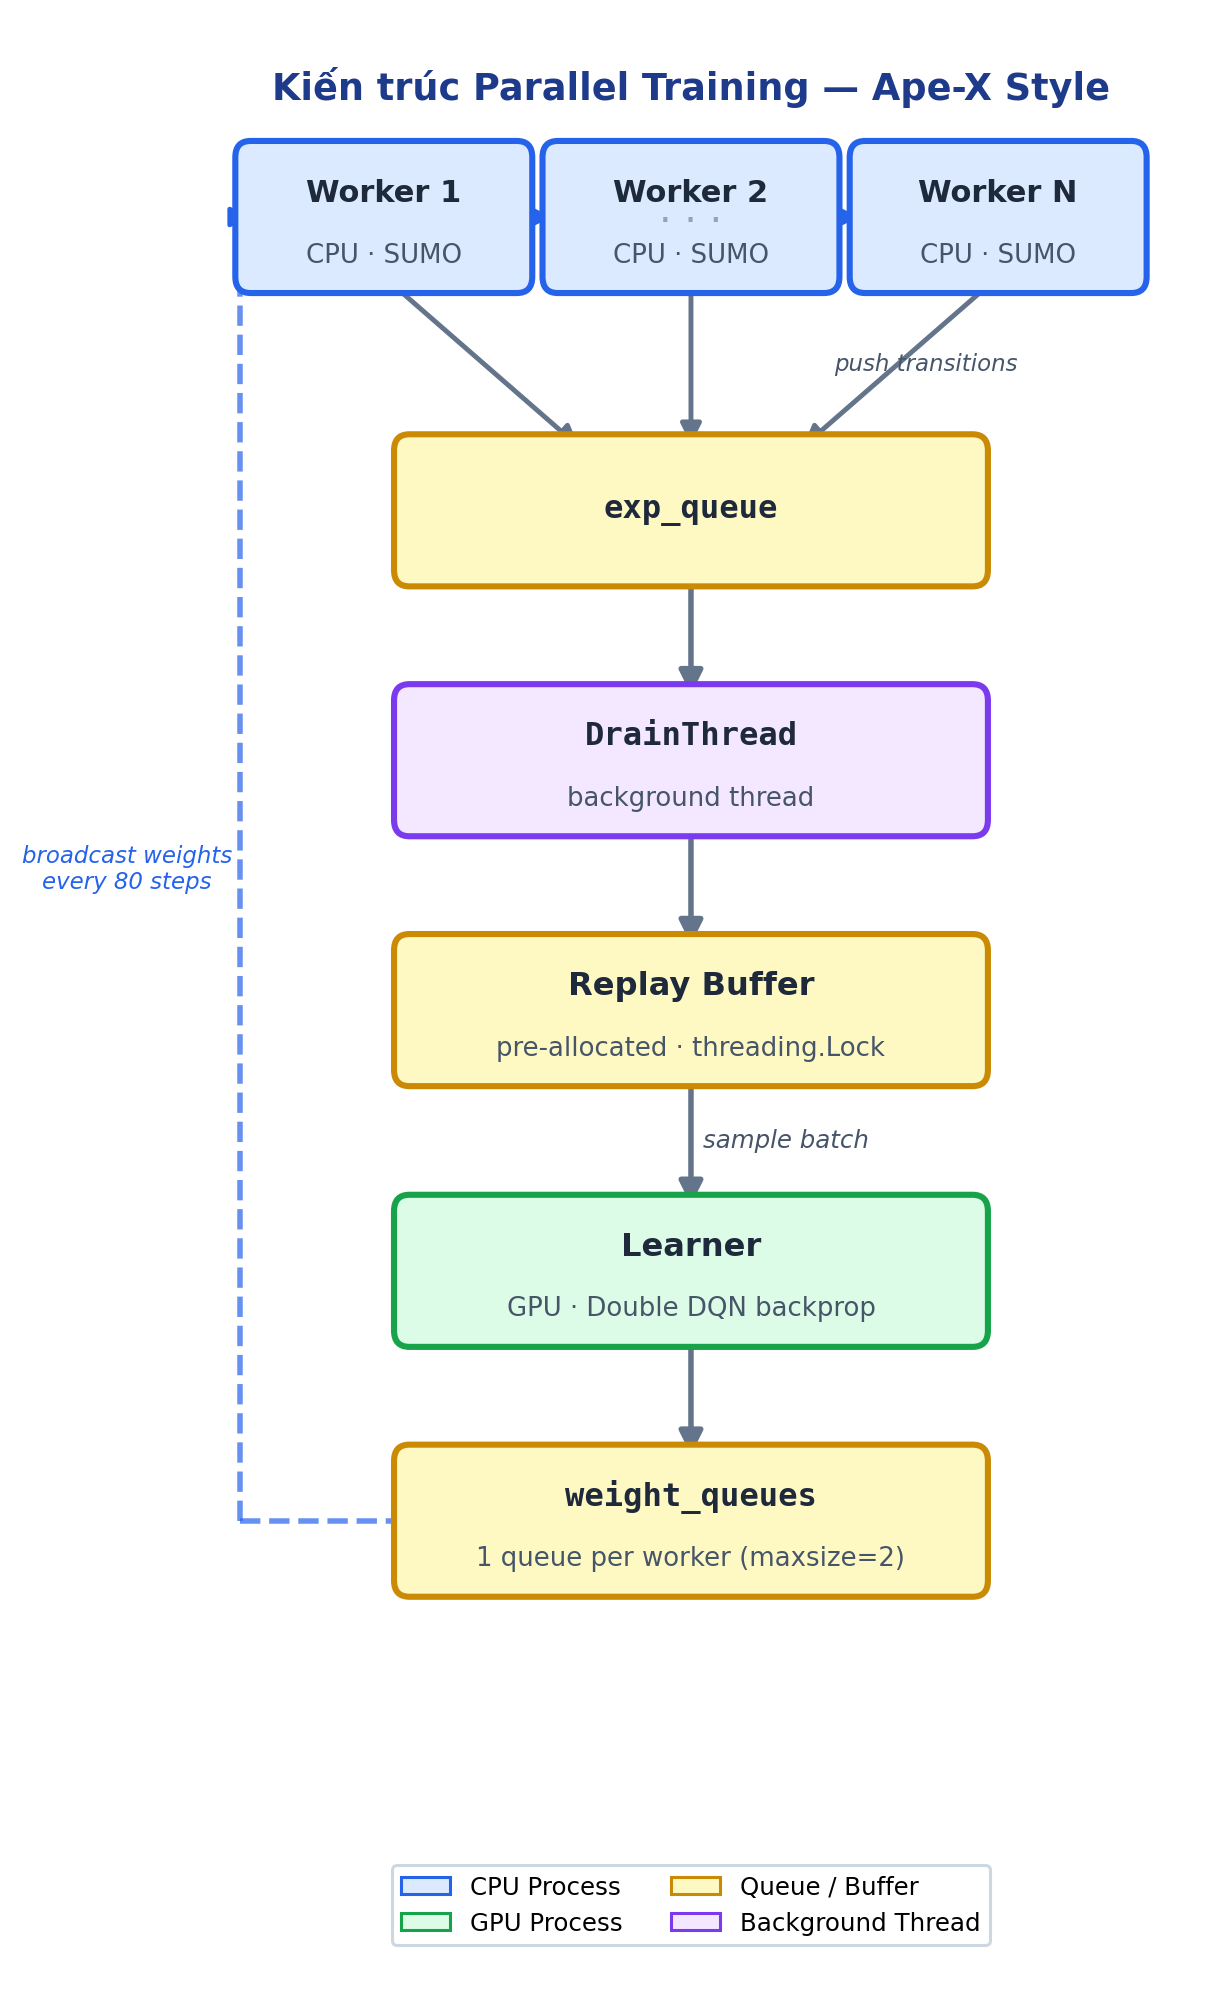
\includegraphics[width=\linewidth]{imgs/apex_diagram.png}
    \caption{Kiến trúc parallel training. Workers chạy SUMO trên CPU, Learner update trên GPU. DrainThread tách riêng để không bị block bởi backprop.}
    \label{fig:parallel}
\end{figure}

\textbf{Fixed-role epsilon workers}: thay vì decay epsilon giống nhau, mỗi worker giữ epsilon \textit{cố định} suốt training, chia đều khoảng $[\varepsilon_{\max}, \varepsilon_{\min}]$:
\begin{equation}
    \varepsilon_k = \varepsilon_{\max} - \frac{(\varepsilon_{\max} - \varepsilon_{\min}) \cdot k}{K - 1}, \quad k = 0, 1, \ldots, K-1
    \label{eq:fixed_eps}
\end{equation}
Worker $k=0$ (explorer, $\varepsilon=1.0$) tạo dữ liệu phủ rộng state space; worker $k=K-1$ (near-greedy, $\varepsilon=0.1$) tạo on-policy experience. Buffer luôn đa dạng từ đầu đến cuối training.

Khác với Ape-X gốc~\cite{ApeX2018} --- nơi các worker có tốc độ epsilon decay khác nhau nhưng đều dần hội tụ về mức thấp --- trong hệ thống này mỗi worker giữ epsilon \textbf{cố định suốt toàn bộ quá trình training} (\texttt{epsilon\_decay=1.0}, \texttt{epsilon\_min=epsilon\_start}). Nhờ đó replay buffer luôn duy trì hỗn hợp ổn định giữa exploration và exploitation từ đầu đến cuối.

Hệ quả của thiết kế fixed-role: replay buffer \textit{luôn} chứa một \textbf{hỗn hợp ổn định} giữa:
\begin{itemize}[leftmargin=*]
    \item \textbf{High-exploration data} (worker $k=0$, $\varepsilon=1.0$): random action, phủ rộng state space, phát hiện trạng thái hiếm gặp.
    \item \textbf{Balanced data} (worker $k$ trung gian): cân bằng explore/exploit, tạo transition đa dạng về chất lượng action.
    \item \textbf{Near-greedy data} (worker $k=K-1$, $\varepsilon=0.1$): gần như pure policy, cung cấp on-policy experience giúp learner thấy phân phối mà policy thực sự gặp khi deploy.
\end{itemize}

Thiết kế này tránh được vấn đề \textbf{distribution shift} phổ biến trong single-worker training: early episodes toàn noise (random actions) dẫn đến buffer chứa data kém chất lượng; late episodes toàn greedy dẫn đến buffer thiếu diversity --- cả hai đều gây instability cho off-policy learning.

\subsection{Replay Buffer}

Pre-allocated numpy circular buffer với threading lock:
\begin{itemize}[leftmargin=*]
    \item Capacity: 50{,}000 transitions.
    \item Schema: $(\mathbf{s}, \mathbf{a}, \mathbf{r}, \mathbf{s}', d)$ với $\mathbf{s} \in \mathbb{R}^{N \times d_s}$.
    \item Lock guard: \texttt{threading.Lock} bảo vệ \texttt{push()} vs \texttt{sample()} khi buffer wrap around --- cần thiết vì phép \texttt{nonlocal int += 1} trong Python không đảm bảo atomic trên bytecode level (\texttt{LOAD\_DEREF} $\to$ \texttt{IADD} $\to$ \texttt{STORE\_DEREF}), tránh race condition khi drain thread và learner cùng truy cập buffer.
    \item \texttt{sample()} copy data ra khỏi lock scope để tránh race condition.
\end{itemize}

\subsection{Update-to-Data Ratio}

Learner kiểm soát tốc độ update bằng ratio: $U_{\text{allowed}} = T_{\text{pushed}} \times R$ với $R = 8$. Mỗi transition được replay $\sim$8 lần trước khi data mới đến --- an toàn cho off-policy DQN. Counter \texttt{\_transitions\_pushed} riêng biệt (không dùng \texttt{len(buffer)}) để tránh bị cap khi buffer đầy.

\subsection{Learning Rate Schedule}

WarmupScheduler: linear warmup 10\% đầu rồi cosine decay:
\begin{equation}
    \text{lr}(t) = \begin{cases}
        \text{lr}_{\text{base}} \cdot \frac{t}{T_w} & t \leq T_w \\[0.5em]
        \text{lr}_{\text{base}} \cdot \frac{1}{2}\left(1 + \cos\left(\pi \cdot \frac{t - T_w}{T - T_w}\right)\right) & t > T_w
    \end{cases}
    \label{eq:lr_schedule}
\end{equation}
với $T_w = T / 10$, lr floor $= 10^{-5}$.

\textbf{Tương tác với 2-phase fine-tuning}: khi finetune, optimizer state được reset hoàn toàn (momentum, second moment của Adam bị xóa), kéo theo scheduler cũng restart từ đầu. Nhờ đó, Phase~1 (freeze GAT) bắt đầu với learning rate thấp từ warmup --- tránh gradient spike khi chỉ Q-head được cập nhật. Đến Phase~2 (unfreeze toàn bộ), scheduler đã qua warmup và bắt đầu cosine decay, giúp GAT layer được fine-tune với learning rate ổn định hơn.

\subsection{Chiến lược Finetune}
\label{sec:finetune}

GAT-MARL hỗ trợ \textbf{2-phase fine-tuning} khi chuyển sang map mới hoặc scenario có vật cản (obstacle), cho phép tận dụng knowledge đã học mà không cần train lại từ đầu.

\textbf{Phase 1 --- Freeze GAT} (\texttt{freeze\_gat\_episodes} episode đầu, mặc định 20): toàn bộ tham số GAT layer bị đóng băng (\texttt{requires\_grad=False}), chỉ Q-head được cập nhật gradient. Lý do: GAT đã học được \textit{graph topology knowledge} --- cách aggregate thông tin từ neighbors --- từ quá trình training gốc. Kiến thức này có tính tổng quát cao, không phụ thuộc vào distribution cụ thể của traffic flow. Do đó, chỉ cần re-calibrate Q-values (output layer) cho distribution mới là đủ.

\textbf{Phase 2 --- Unfreeze toàn bộ} (sau \texttt{freeze\_gat\_episodes}): toàn bộ network được unfreeze và tiếp tục train với learning rate thấp (đã qua warmup), cho phép GAT fine-tune attention weights cho topology/scenario mới.

IDQN không có communication layer tách biệt --- toàn bộ network là một khối MLP đồng nhất, không có module nào mang tính tổng quát riêng. Khi chuyển sang map hoặc scenario mới, IDQN phải train lại từ đầu trong khi GAT-MARL chỉ cần fine-tune.

\textbf{Cơ chế load checkpoint}:
\begin{itemize}[leftmargin=*]
    \item \texttt{finetune=True}: chỉ load weights (warm-start), \textit{reset} optimizer state và giữ \texttt{epsilon\_start} cao để agent explore map mới. Optimizer bắt đầu với momentum sạch, tránh bị kéo theo hướng gradient cũ.
    \item \texttt{resume=True}: load toàn bộ state (weights + optimizer + epsilon + update counter), tiếp tục training chính xác từ điểm dừng trước.
\end{itemize}

Log file được mở ở mode \texttt{"a"} (append) khi finetune hoặc resume, đảm bảo không mất training history từ các phase trước. Mode \texttt{"w"} (overwrite) chỉ dùng khi fresh training.

\subsection{Double DQN Target}

Bellman target cho tất cả $N$ agents trong batch:
\begin{equation}
    y_{b,i} = r_{b,i} + \gamma \cdot Q_{\theta^{-}}\!\left(\mathbf{s}'_{b,i},\, \arg\max_a Q_\theta(\mathbf{s}'_{b,i}, a)\right) \cdot (1 - d_b)
    \label{eq:target}
\end{equation}
Done signal $d_b$ là centralized (episode kết thúc đồng thời cho tất cả agents), broadcast $(\text{B}) \to (\text{B}, N)$.

Loss: Huber Loss (\texttt{SmoothL1Loss}) với gradient clipping $\|\nabla\| \leq 10.0$.

% ══════════════════════════════════════════════════════════════════════════════
%  6. CÁC CẢI TIẾN KỸ THUẬT
% ══════════════════════════════════════════════════════════════════════════════
\section{Các cải tiến kỹ thuật}

\subsection{Reward Normalization}

Cả waiting time và pressure đều được normalize về $[0, 1]$ \textit{trước} khi nhân $\alpha, \beta$, đảm bảo hai thành phần có cùng scale:
\begin{itemize}[leftmargin=*]
    \item Waiting time clip tại $W_{\max} = 120$s (2 phút --- tương đương LOS~F theo HCM).
    \item Pressure clip tại $P_{\max} = 5.0$ (queue max $\sim$20 xe / 4 lanes).
\end{itemize}
Không normalize, pressure (đơn vị: xe) và waiting time (đơn vị: giây) sẽ có magnitude rất khác, khiến $\alpha, \beta$ không còn ý nghĩa 70--30.

\textbf{Ví dụ định lượng}: xét một ngã tư có $\bar{w} = 80$s (waiting time trung bình) và $p = 3.2$ (pressure):

\textit{Không normalize} --- áp dụng trực tiếp $\alpha, \beta$ lên raw values:
\begin{equation*}
    r = -\left(0.7 \times 80 + 0.3 \times 3.2\right) = -(56.0 + 0.96) = -56.96
\end{equation*}
Thành phần waiting time đóng góp $56.0$, pressure đóng góp $0.96$ --- tỉ lệ thực tế là $\mathbf{98{:}2}$ thay vì 70{:}30 như thiết kế. Pressure gần như bị \textit{triệt tiêu hoàn toàn}.

\textit{Có normalize} ($W_{\max}=120$, $P_{\max}=5$):
\begin{align*}
    \hat{w} &= 80 / 120 = 0.667 \\
    \hat{p} &= 3.2 / 5 = 0.640 \\
    r &= -(0.7 \times 0.667 + 0.3 \times 0.640) \times 5 \\
      &= -(0.467 + 0.192) \times 5 = -3.29
\end{align*}
Thành phần waiting time đóng góp $0.467 \times 5 = 2.33$, pressure đóng góp $0.192 \times 5 = 0.96$ --- tỉ lệ thực tế là $\mathbf{71{:}29}$, gần đúng với $\alpha{:}\beta = 70{:}30$.

Như vậy, normalize đảm bảo $\alpha$ và $\beta$ phản ánh đúng tỉ lệ đóng góp mong muốn giữa hai thành phần reward, thay vì trở thành hệ số nhân vô nghĩa trên hai đại lượng khác đơn vị.

\subsection{Teleport Penalty Capping}

Teleport penalty ban đầu unbounded, có thể gấp 3 lần base reward khi gridlock. Giá trị được cap tại 2.5 ($= 50\%$ base reward range) để tránh gradient spike tạm thời.

\subsection{Dynamic Lane Detection}

Hàm \texttt{get\_edge\_lanes()} trả về số lane thực tế cho từng edge thay vì dùng giá trị mặc định. Trên map Mỹ Đình, arterial (Hồ Tùng Mậu) có 3 lanes, secondary (Hàm Nghi) có 2 lanes --- detector subscription và state builder đều sử dụng giá trị thực này.

\subsection{Cooperative Shared Reward}

GAT-MARL dùng hybrid reward $r_i^{\text{train}} = 0.7 \cdot r_i + 0.3 \cdot \bar{r}$ (với $\bar{r} = \text{mean}(r_1, \ldots, r_N)$) để vừa giữ tín hiệu phân biệt per-agent vừa khuyến khích cooperative behavior, nhất quán với communication qua GAT. IDQN giữ individual reward vì không có cơ chế coordination.

\textbf{Lưu ý phân biệt}: hàm \texttt{compute\_global\_reward()} trong \texttt{reward.py} tính tổng reward toàn mạng và chỉ dùng cho \textbf{logging/evaluation} (ghi vào CSV để theo dõi tiến trình). Signal dùng để \textbf{train} là shared reward được tính ở tầng worker loop trong \texttt{train\_parallel.py} --- hai giá trị này nhất quán về ý nghĩa nhưng tách biệt về vai trò.

\subsection{Route Distribution}

Mỗi episode lấy ngẫu nhiên kịch bản \texttt{peak\_morning} (35\%), \texttt{peak\_evening} (35\%), hoặc \texttt{night} (30\%). Volume có thể scale từ $0.5\times$ đến $1.8\times$ để mô phỏng các mức lưu lượng khác nhau.

\subsection{Obstacle Injection}

Mô phỏng sự cố thực tế (công trình, xe hỏng) bằng cách inject 1--3 vật cản đồng thời vào random edges. Block mode: \texttt{all} (disallow toàn bộ vehicle class) hoặc \texttt{left/right} (giảm maxSpeed xuống 0.3 m/s). Original maxSpeed được cache để restore chính xác.

\subsection{Temp File Cleanup}

Khi scale volume, file route tạm được tạo với \texttt{delete=False} và dọn dẹp tự động trong \texttt{reset()} và \texttt{close()}, tránh disk leak qua nhiều episodes.

% ══════════════════════════════════════════════════════════════════════════════
%  7. THỰC NGHIỆM VÀ KẾT QUẢ
% ══════════════════════════════════════════════════════════════════════════════
\section{Thực nghiệm và kết quả}

\subsection{Cấu hình thực nghiệm}

\textbf{Phần cứng}: Laptop gaming với CPU AMD Ryzen 7-6800H, RAM 16GB. Kiến trúc parallel tận dụng cả hai: CPU chạy các SUMO worker process song song để sinh experience, GPU đảm nhận backpropagation cho Learner.

\textbf{Hyperparameters}: Bảng~\ref{tab:hyperparams} tóm tắt các tham số chính.

\begin{table}[h]
\centering
\caption{Hyperparameters chính}
\label{tab:hyperparams}
\begin{tabular}{lrl}
\toprule
\textbf{Tham số} & \textbf{Giá trị} & \textbf{Ghi chú} \\
\midrule
Learning rate & $10^{-4}$ & Adam optimizer \\
$\gamma$ (discount) & 0.95 & $Q \in [-100, 0]$ \\
Batch size & 64 & \\
Replay buffer & 50{,}000 & Circular, pre-allocated \\
Target update & 400 & Gradient updates \\
Hidden dim & 64 & Encoder + Q-head \\
GAT heads & 4 & \texttt{concat=False} \\
Grad clip & 10.0 & Max norm \\
Reward scale $S$ & 5.0 & \\
$\alpha / \beta$ & 0.7 / 0.3 & Wait / Pressure \\
Workers & 2 & Default \texttt{train\_parallel} \\
$\Delta t$ & 5s & Decision interval \\
SIM\_END & 1800s & 30 phút/episode \\
Min replay size & 1{,}000 & Warm-start trước khi update \\
UTD ratio $R$ & 8 & Updates per transition \\
\bottomrule
\end{tabular}
\end{table}

\subsection{Kết quả training}

% ┌──────────────────────────────────────────────────────┐
% │ [TODO] Chèn learning curves (reward, loss, epsilon)  │
% │ → export từ dashboard Results tab hoặc matplotlib    │
% └──────────────────────────────────────────────────────┘

\begin{figure}[h]
    \centering
    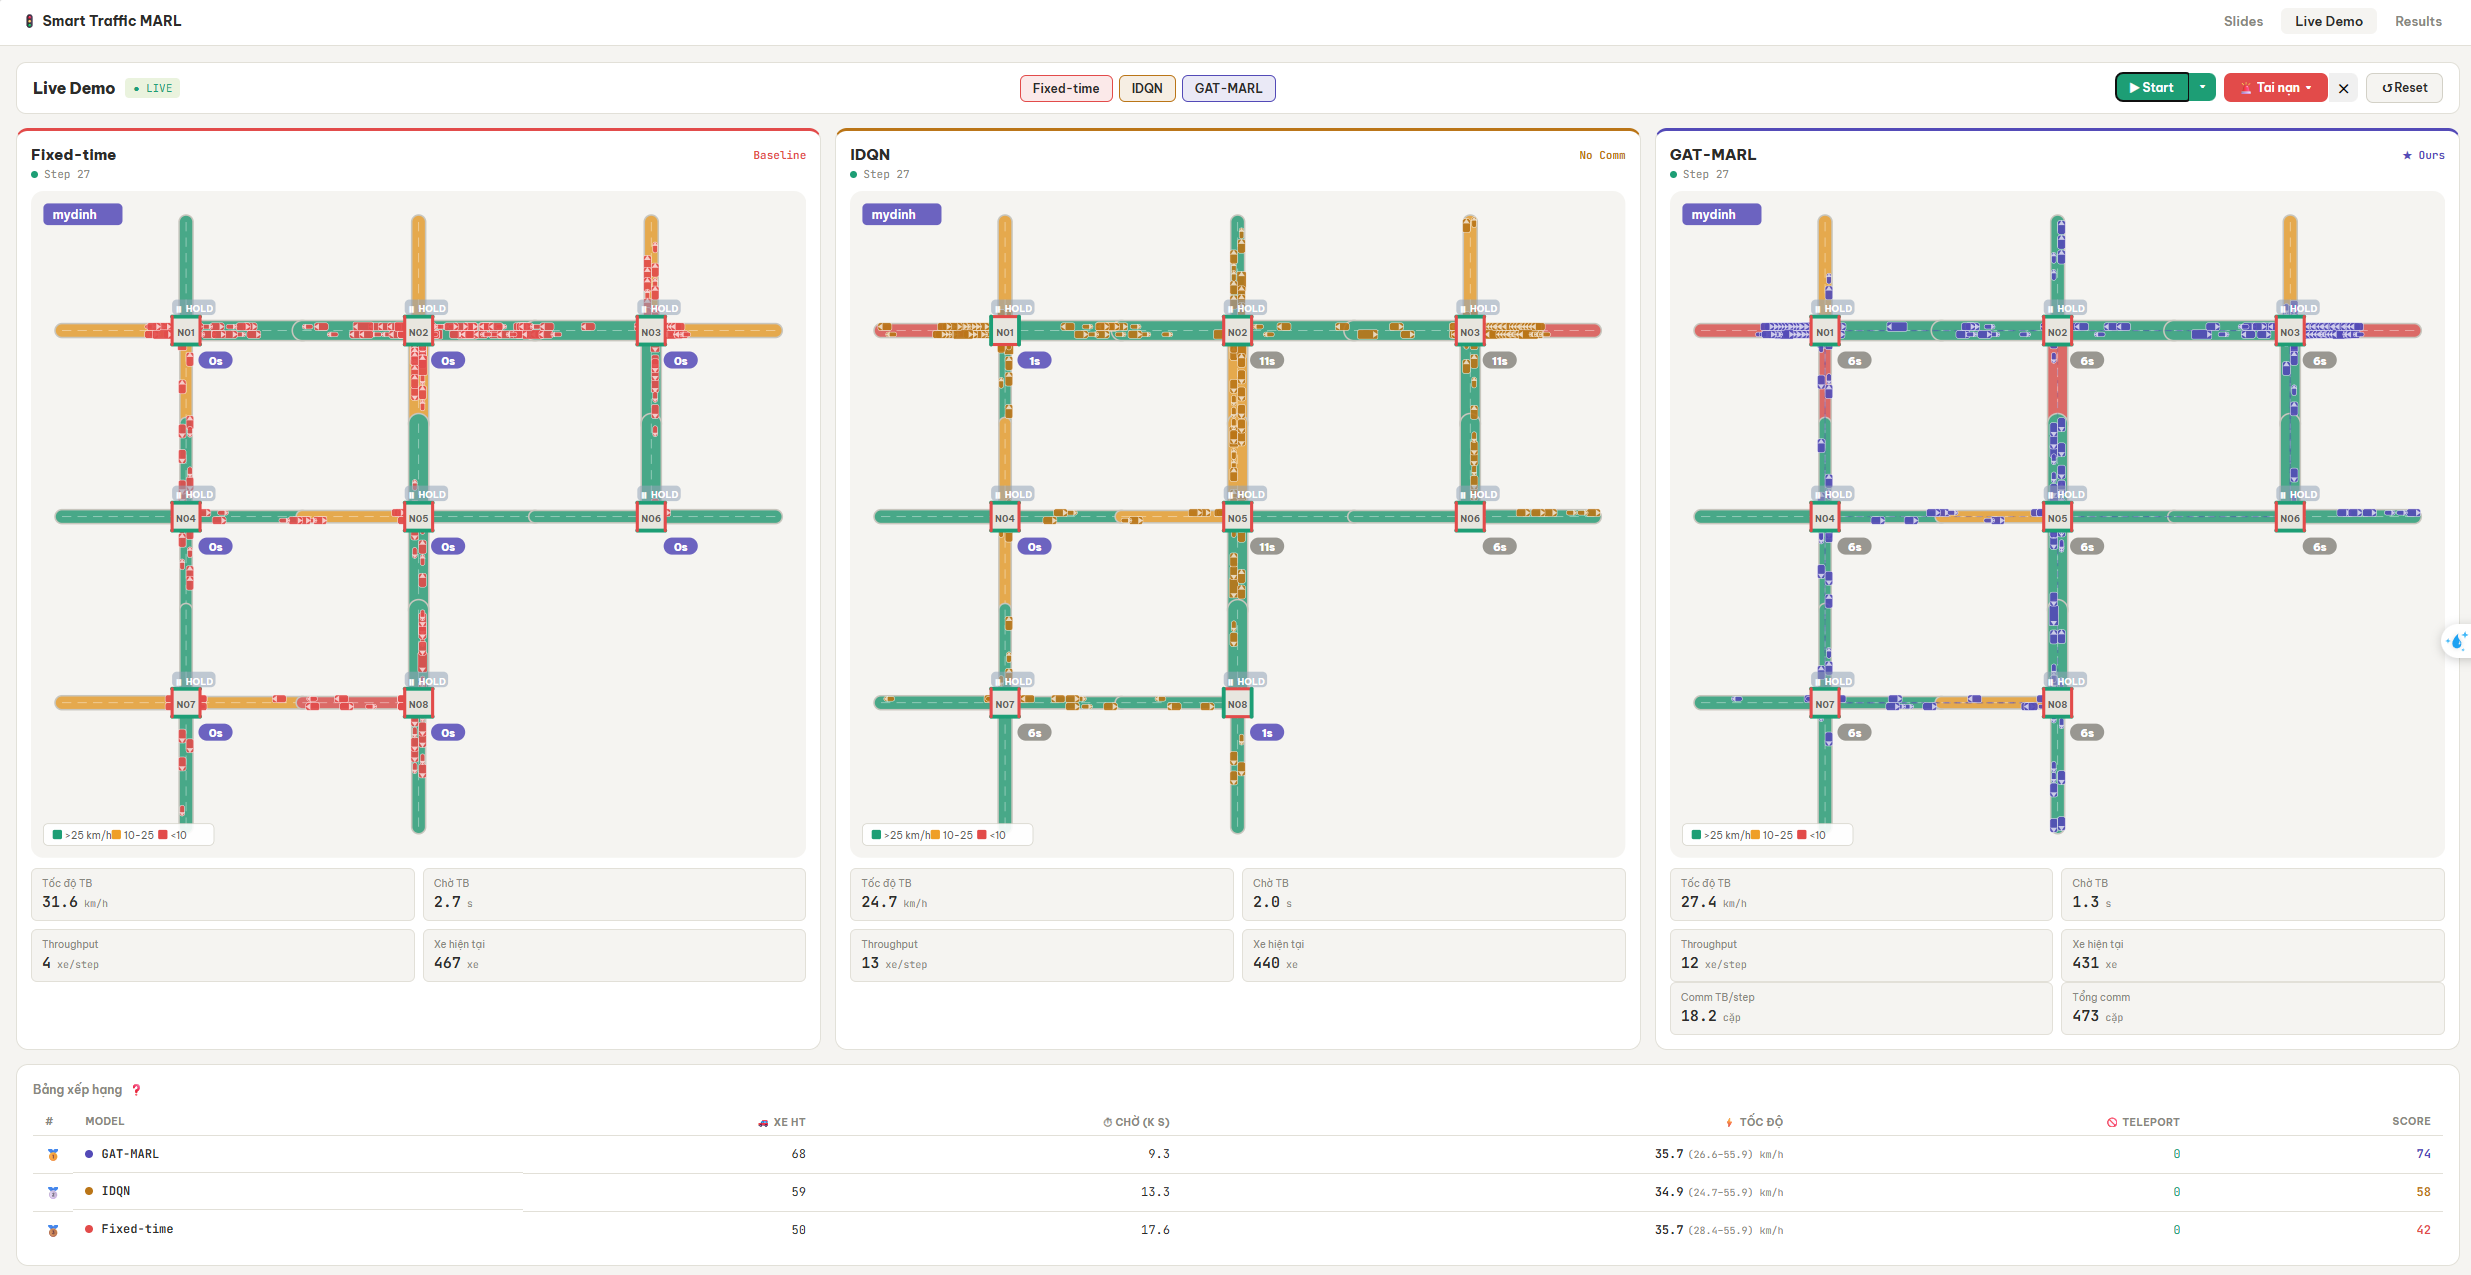
\includegraphics[width=\linewidth]{imgs/live_demo_mydinh.png}
    \caption{Learning curves so sánh GAT-MARL, IDQN, và Fixed-time trên map Mỹ Đình (500 episodes, parallel training 2 workers).}
    \label{fig:learning_curves}
\end{figure}

\subsection{So sánh mô hình}

% ┌──────────────────────────────────────────────────────────┐
% │ [TODO] Điền số liệu thực nghiệm từ logs/merged.json    │
% │ Lấy 50 episodes cuối cùng để tính mean ± std            │
% └──────────────────────────────────────────────────────────┘

\begin{table}[h]
\centering
\caption{So sánh hiệu năng 3 phương pháp (50 episodes cuối, map Mỹ Đình)}
\label{tab:results}
\setlength{\tabcolsep}{4pt}
\begin{tabular}{lp{1.6cm}p{1.6cm}p{1.6cm}}
\toprule
\textbf{Metric} & \textbf{Fixed} & \textbf{IDQN} & \textbf{GAT-MARL} \\
\midrule
Avg Wait (s) $\downarrow$      & $5.18 \pm 4.09$  & $3.99 \pm 3.83$   & $4.46 \pm 4.20$ \\
Avg Speed (km/h) $\uparrow$    & $18.90 \pm 7.82$ & $21.91 \pm 11.12$ & $18.68 \pm 9.81$ \\
Throughput $\uparrow$          & $2251 \pm 902$   & $1829 \pm 823$    & $1946 \pm 746$ \\
Teleport $\downarrow$          & $0.00$           & $0.00$            & $0.00$ \\
Reward $\uparrow$              & $-363.6 \pm 217.4$  & $-260.0 \pm 171.8$   & $-340.2 \pm 312.1$ \\
\bottomrule
\end{tabular}
\end{table}

\subsection{Khả năng thích ứng sự cố}

% ┌──────────────────────────────────────────────────────────┐
% │ [TODO] So sánh reward khi có/không có obstacle          │
% └──────────────────────────────────────────────────────────┘

\begin{table}[h]
\centering
\caption{Hiệu năng khi có vật cản (obstacle\_prob = 0.4)}
\label{tab:obstacle}
\setlength{\tabcolsep}{4pt}
\begin{tabular}{lp{1.5cm}p{1.5cm}p{1.6cm}}
\toprule
& \textbf{Fixed} & \textbf{IDQN} & \textbf{GAT-MARL} \\
\midrule
Reward (no obs)   & $-300.6 \pm 77.3$  & $-222.1 \pm 74.2$  & $-238.9 \pm 63.8$ \\
Reward (with obs) & $-458.0 \pm 311.6$ & $-348.5 \pm 279.1$ & $-480.0 \pm 444.4$ \\
$\Delta$ Reward   & $-157.4$           & $-126.4$           & $-241.1$ \\
\bottomrule
\end{tabular}
\end{table}

\subsection{GAT Attention Visualization}

% ┌──────────────────────────────────────────────────────────┐
% │ [TODO] Screenshot attention heatmap từ dashboard        │
% └──────────────────────────────────────────────────────────┘

\begin{figure}[h]
    \centering
    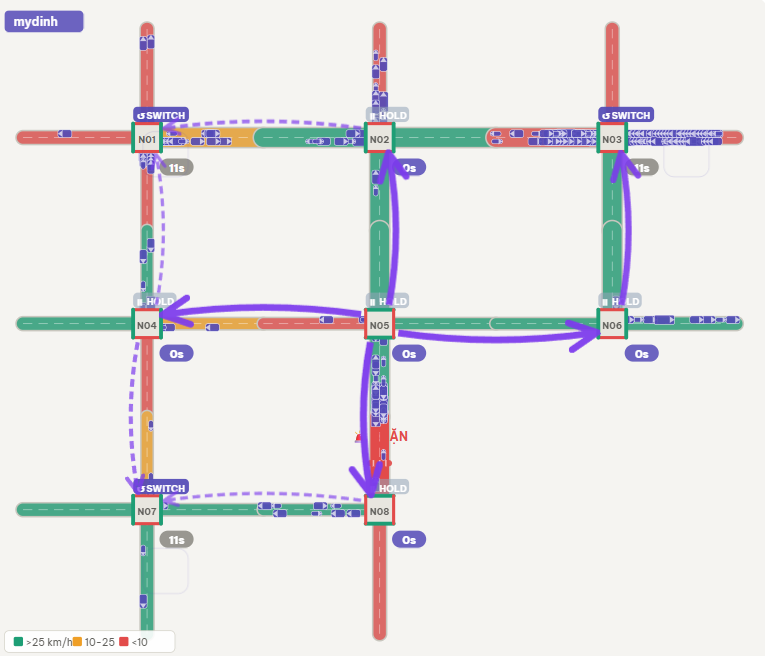
\includegraphics[width=\linewidth]{imgs/attention_mydinh.png}
    \caption{Attention weights giữa 8 ngã tư tại một thời điểm peak traffic. Giá trị cao (đậm) cho thấy agent $i$ chú ý mạnh đến neighbor $j$.}
    \label{fig:attention}
\end{figure}

\subsection{Khả năng chuyển giao sang map UET}

% ┌──────────────────────────────────────────────────────────────────┐
% │ [TODO] Điền số liệu episodes/thời gian finetune GAT-MARL vs    │
% │        training from scratch IDQN trên map UET                  │
% └──────────────────────────────────────────────────────────────────┘

Để đánh giá khả năng generalization, hệ thống được kiểm chứng trên map \textbf{UET} --- khu vực Đại học Công nghệ, Cầu Giấy (Hình~\ref{fig:uet_topology}), phức tạp hơn đáng kể với \textbf{15 ngã tư} (N01--N15). Mạng lưới gồm 2 trục arterial ngang (Hồ Tùng Mậu -- Row 1, Trịnh Văn Bô/Trần Hữu Dực -- Row 2), 3 trục arterial dọc (Xuân Phương, Phạm Hùng, và một phần Hồ Tùng Mậu kéo dài), và các đường secondary nội bộ (Hàm Nghi, Kiều Mai, Nguyễn Văn Giáp, Nguyễn Cơ Thạch, Lê Đức Thọ).

\begin{figure}[!t]
    \centering
    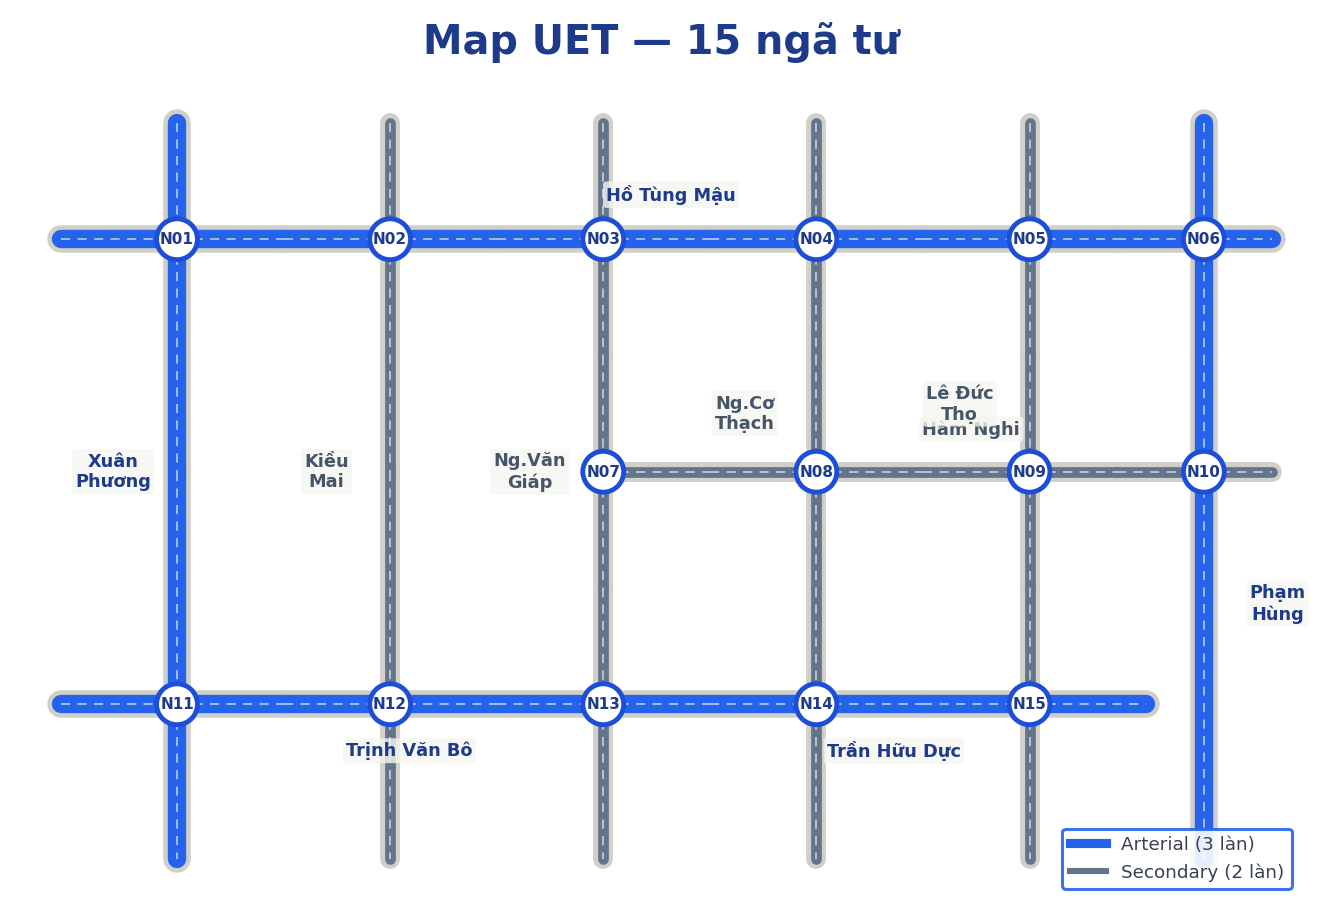
\includegraphics[width=\linewidth]{imgs/map_uet.png}
    \caption{Topology mạng lưới giao thông khu vực UET (15 ngã tư).}
    \label{fig:uet_topology}
\end{figure}

\begin{table}[!t]
\centering
\caption{So sánh hiệu năng và hội tụ trên map UET (15 ngã tư, 50 eps cuối)}
\label{tab:transfer}
\setlength{\tabcolsep}{4pt}
\begin{tabular}{p{2.0cm} c c p{1.8cm}}
\toprule
\textbf{Phương pháp} & \textbf{Eps hội tụ} & \textbf{Reward} & \textbf{Chiến lược} \\
\midrule
GAT-MARL (finetune) & \textbf{6}  & $-648.4 \pm 320.3$ & Freeze/unfreeze 2-phase \\
IDQN (scratch)      & 43          & $-689.1 \pm 324.5$ & Train lại từ đầu \\
Fixed-time          & ---         & $-767.7 \pm 300.8$ & Không học \\
\bottomrule
\end{tabular}
\end{table}

GAT-MARL tận dụng checkpoint từ Mỹ Đình qua cơ chế \textbf{2-phase fine-tuning} (Section~\ref{sec:finetune}): GAT layer giữ lại \textit{graph topology knowledge} đã học --- cách aggregate thông tin từ neighbors --- và chỉ cần re-calibrate Q-head cho distribution mới. IDQN không có communication layer tách biệt nên phải train lại từ đầu, dẫn đến thời gian hội tụ dài hơn đáng kể trên mạng 15 ngã tư.

\subsection{Dashboard Giám sát Real-time}

Hệ thống đi kèm dashboard web real-time (FastAPI + WebSocket backend, React + Vite frontend) cho phép quan sát và so sánh trực tiếp ba phương pháp \textbf{Fixed-time}, \textbf{IDQN}, và \textbf{GAT-MARL} chạy song song trên cùng một episode SUMO (Hình~\ref{fig:dashboard}).

\begin{figure}[h]
    \centering
    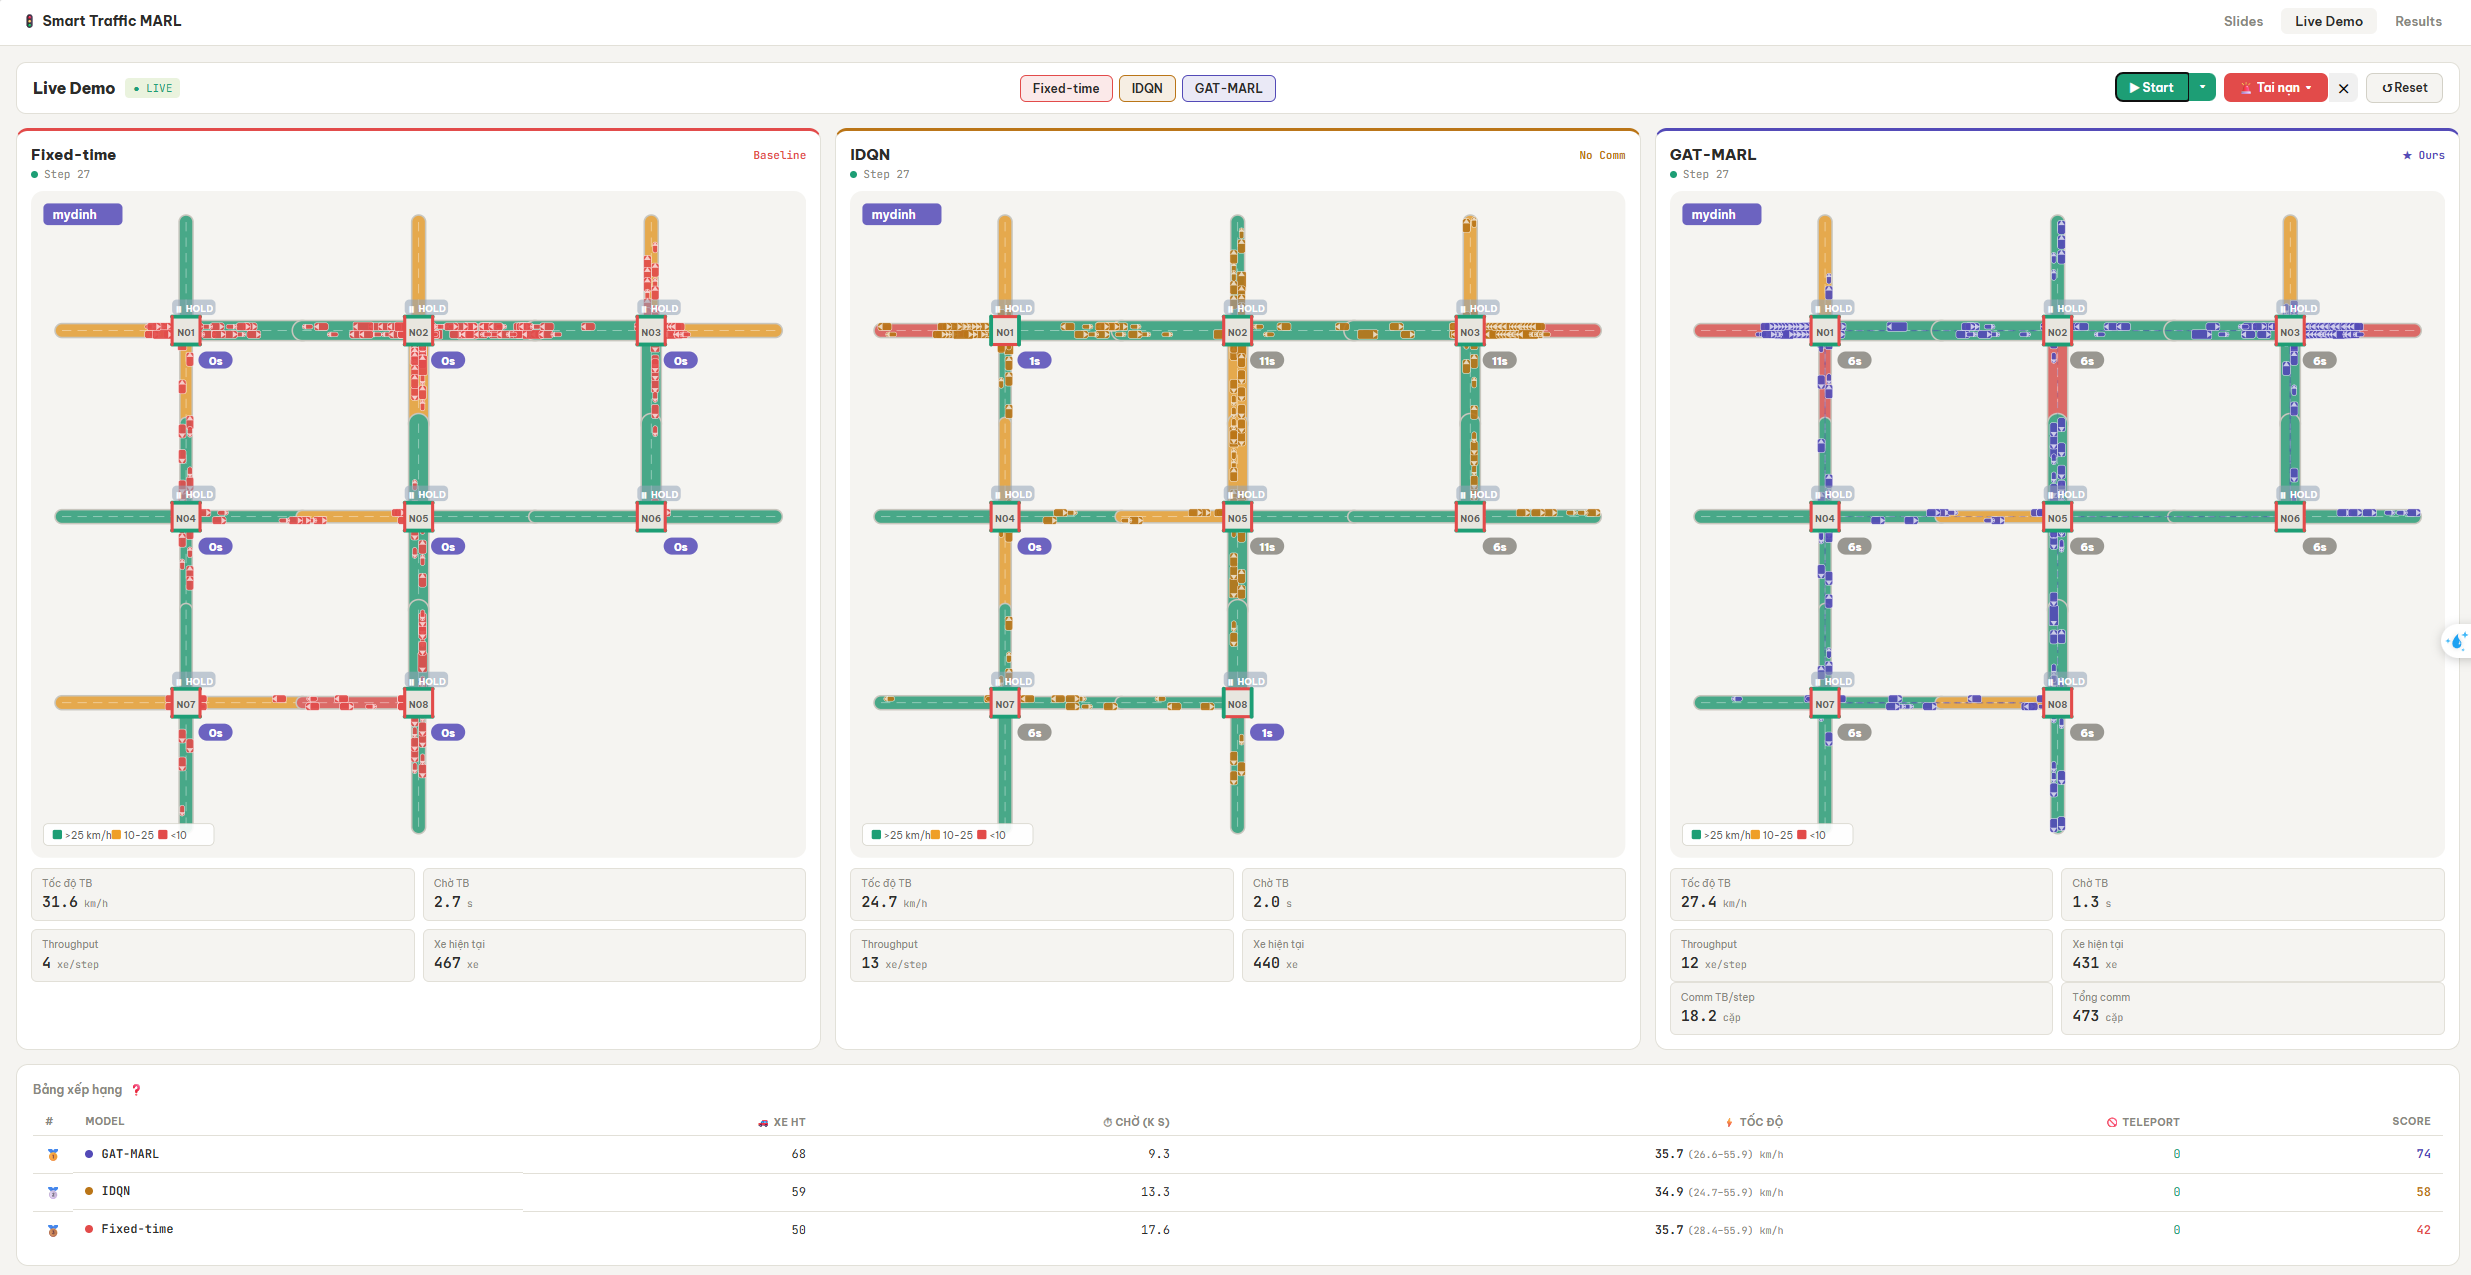
\includegraphics[width=\linewidth]{imgs/live_demo_mydinh.png}
    \caption{Dashboard real-time trên map Mỹ Đình: ba phương pháp (Fixed-time, IDQN, GAT-MARL) chạy song song, hiển thị reward tích lũy, tốc độ trung bình, và trạng thái từng ngã tư theo thời gian thực.}
    \label{fig:dashboard}
\end{figure}

Dashboard cập nhật qua WebSocket mỗi decision step ($\Delta t = 5$s), hiển thị các metric: global reward tích lũy, average speed (km/h), waiting time trung bình, và số lần teleport. Tab \textit{Attention Viewer} hiển thị attention heatmap $N \times N$ từ GAT layer sau mỗi forward pass, cho phép quan sát trực quan agent nào đang chú ý đến neighbor nào tại thời điểm traffic cao.

% ══════════════════════════════════════════════════════════════════════════════
%  8. THẢO LUẬN
% ══════════════════════════════════════════════════════════════════════════════
\section{Thảo luận}

\textbf{Phân tích hiệu năng GAT-MARL so với IDQN}: kết quả thực nghiệm trên map Mỹ Đình cho thấy GAT-MARL (Global Reward $-340$) chưa vượt được IDQN ($-260$) sau 500 episodes, dù cả hai đều tốt hơn Fixed-time ($-364$). Phân tích training dynamics chỉ ra hai nguyên nhân chính, có căn cứ từ log:

\textit{(1) Credit assignment bất ổn do hybrid reward}: GAT-MARL dùng reward $0.7 r_i + 0.3\bar{r}$. Trong các episodes có obstacle (30\% tổng số), $\bar{r}$ giảm sâu kéo theo Q-values của toàn bộ agents, gây loss spike và reward âm cực đoan (min $= -1525$ so với $-882$ của IDQN). Điều này giải thích tại sao reward GAT-MARL có phân phối bimodal: một số episodes rất tốt ($\sim -113$, tương đương IDQN) nhưng xen kẽ các episodes thảm họa.

\textit{(2) GAT chưa ổn định trên graph nhỏ}: với chỉ $N=8$ ngã tư, attention mechanism ít không gian để differentiate --- 4 heads có thể học các pattern trùng lặp. Biểu hiện: loss GAT vẫn tăng đều (0.005 $\to$ 0.032) sau 500 episodes trong khi reward không cải thiện, cho thấy model đang overfit vào một số neighbor patterns thay vì generalize. Đây cũng lý giải tại sao GAT-MARL lại hội tụ rất nhanh trên UET (15 ngã tư) --- graph đủ lớn để attention có ý nghĩa hơn.

Kết quả chuyển giao sang UET (GAT hội tụ ep~6 vs IDQN ep~43, nhanh hơn 7×) xác nhận rằng kiến trúc GAT-MARL học được \textit{cấu trúc graph} tốt, nhưng cần graph đủ phức tạp để phát huy. Hướng khắc phục: tăng số episodes training, bổ sung prioritized experience replay để giảm ảnh hưởng của obstacle episodes cực đoan.

\textbf{Parameter sharing}: toàn bộ agents dùng chung 1 bộ trọng số (encoder, GAT, Q-head). Ưu điểm: (1) giảm $N\times$ số tham số cần học, (2) transfer learning tự nhiên khi thêm/bớt ngã tư, (3) mỗi transition huấn luyện cho tất cả agents. Nhược điểm: agent không có identity riêng --- GAT layer phần nào khắc phục bằng cách differentiate qua graph topology.

\textbf{Reward design}: hybrid waiting time + pressure hoạt động tốt hơn pure pressure vì waiting time phản ánh trực tiếp trải nghiệm người dùng, trong khi pressure giữ vai trò regularizer tránh spillback. Normalize về $[0, 1]$ trước khi kết hợp đảm bảo $\alpha, \beta$ thực sự phản ánh tỉ lệ mong muốn.

\textbf{Trade-off của hybrid reward}: thiết kế $0.7 \cdot r_i + 0.3 \cdot \bar{r}$ là kết quả của sự đánh đổi giữa \textit{coordination} và \textit{credit assignment}. Pure shared reward ($\bar{r}$ thuần túy) tối đa hóa coordination nhưng làm mờ tín hiệu: mỗi agent không phân biệt được khi hành động của mình tốt hay kém, dẫn đến Q-values của các ngã tư có cùng neighbors hội tụ về nhau và gradient hiệu quả bị triệt tiêu. Ngược lại, pure individual reward không tận dụng được communication layer. Hệ số 0.7/0.3 giữ 70\% tín hiệu per-agent để Q-values vẫn differentiate được giữa các ngã tư, đồng thời 30\% global mean cung cấp cooperative signal đủ để GAT attention weights học được pattern phối hợp có ý nghĩa. Tuy nhiên, khi một ngã tư gặp sự cố, $\bar{r}$ giảm vẫn kéo reward các agent khác xuống (dù ít hơn pure shared). Prioritized experience replay (hướng phát triển tiếp theo) có thể giảm thiểu ảnh hưởng này bằng cách ưu tiên sample các transition có TD-error lớn.

\textbf{Hạn chế}: (1) action space chỉ 2 chiều (keep/switch) --- chưa hỗ trợ nhiều phase phức tạp; (2) chưa có prioritized experience replay; (3) chưa kiểm chứng trên mạng lưới lớn hơn 15 ngã tư hoặc kịch bản multi-city.

% ══════════════════════════════════════════════════════════════════════════════
%  9. KẾT LUẬN
% ══════════════════════════════════════════════════════════════════════════════
\section{Kết luận}

Báo cáo trình bày hệ thống GAT-MARL --- kết hợp Graph Attention Network với Multi-Agent Deep Q-Learning --- được xây dựng và kiểm chứng trên hai mạng lưới thực tế: \textbf{Mỹ Đình} (8 ngã tư) và \textbf{UET} (15 ngã tư). Các đóng góp kỹ thuật bao gồm: reward function hybrid với normalization, parallel training với fixed-role epsilon workers, dynamic lane detection, obstacle injection, và cơ chế 2-phase fine-tuning cho phép chuyển giao kiến thức sang topology mới mà không cần train lại từ đầu.

Thực nghiệm trên map Mỹ Đình (50 episodes cuối) cho thấy cả hai phương pháp RL đều vượt trội so với Fixed-time về Global Reward ($-260$ và $-340$ so với $-364$) và Avg Wait ($3.99$s và $4.46$s so với $5.18$s). Thực nghiệm chuyển giao từ Mỹ Đình sang UET cho thấy GAT-MARL hội tụ chỉ sau \textbf{6 episodes} (6.17h) so với IDQN cần \textbf{43 episodes} (15.41h) khi train from scratch, xác nhận giá trị của việc tách biệt communication layer trong thiết kế kiến trúc MARL.

Hướng phát triển tiếp theo: (1) mở rộng lên mạng lưới $>$15 ngã tư, (2) bổ sung prioritized experience replay, (3) thử nghiệm action space đa phase, (4) tích hợp dữ liệu giao thông thực từ camera.

% ══════════════════════════════════════════════════════════════════════════════
%  PHÂN CÔNG CÔNG VIỆC
% ══════════════════════════════════════════════════════════════════════════════
\section*{Phân công công việc}

\begin{table}[!h]
\centering
\small
\begin{tabular}{p{2.8cm} p{5cm}}
\toprule
\textbf{Thành viên} & \textbf{Công việc} \\
\midrule
Đặng Quang Minh
&
Thiết kế kiến trúc GAT-MARL, cài đặt training pipeline, viết báo cáo \\[0.8em]

Ngô Trọng Hiệp
&
Xây dựng môi trường SUMO, thiết kế reward function, thực nghiệm \\[0.8em]

Khổng Quang Huy
&
Xây dựng dashboard, cài đặt IDQN baseline, phân tích kết quả \\
\bottomrule
\end{tabular}
\end{table}

% ══════════════════════════════════════════════════════════════════════════════
%  REFERENCES
% ══════════════════════════════════════════════════════════════════════════════
\begin{thebibliography}{99}

\bibitem{Mnih2015}
V.~Mnih, K.~Kavukcuoglu, D.~Silver, A.~A.~Rusu, J.~Veness, M.~G.~Bellemare, A.~Graves, M.~Riedmiller, A.~K.~Fidjeland, G.~Ostrovski, S.~Petersen, C.~Beattie, A.~Sadik, I.~Antonoglou, H.~King, D.~Kumaran, D.~Wierstra, S.~Legg, and D.~Hassabis,
``Human-level control through deep reinforcement learning,''
\textit{Nature}, vol.~518, no.~7540, pp.~529--533, Feb. 2015.

\bibitem{vanHasselt2016}
H.~van Hasselt, A.~Guez, and D.~Silver,
``Deep reinforcement learning with Double Q-learning,''
in \textit{Proc. AAAI Conf. Artif. Intell.}, 2016.
arXiv:1509.06461.

\bibitem{Velickovic2018}
P.~Veličković, G.~Cucurull, A.~Casanova, A.~Romero, P.~Liò, and Y.~Bengio,
``Graph Attention Networks,''
in \textit{Proc. Int. Conf. Learn. Represent. (ICLR)}, 2018.
arXiv:1710.10903.

\bibitem{PressLight2019}
H.~Wei, C.~Chen, G.~Zheng, K.~Wu, V.~Gayah, K.~Xu, and Z.~Li,
``PressLight: Learning Max Pressure control to coordinate traffic signals in arterial network,''
in \textit{Proc. 25th ACM SIGKDD Int. Conf. Knowl. Discov. Data Mining (KDD)}, 2019, pp.~1290--1298.

\bibitem{CoLight2019}
H.~Wei, N.~Xu, H.~Zhang, G.~Zheng, X.~Zang, C.~Chen, W.~Zhang, Y.~Zhu, K.~Xu, and Z.~Li,
``CoLight: Learning network-level cooperation for traffic signal control,''
in \textit{Proc. 28th ACM Int. Conf. Inf. Knowl. Manag. (CIKM)}, 2019.
arXiv:1905.05717.

\bibitem{MPLight2020}
C.~Chen, H.~Wei, N.~Xu, G.~Zheng, M.~Yang, Y.~Xiong, K.~Xu, and Z.~Li,
``Toward a thousand lights: Decentralized deep reinforcement learning for large-scale traffic signal control,''
in \textit{Proc. 34th AAAI Conf. Artif. Intell.}, 2020.

\bibitem{ApeX2018}
D.~Horgan, J.~Quan, D.~Budden, G.~Barth-Maron, M.~Hessel, H.~van Hasselt, and D.~Silver,
``Distributed prioritized experience replay,''
in \textit{Proc. Int. Conf. Learn. Represent. (ICLR)}, 2018.
arXiv:1803.00933.

\bibitem{SUMO2018}
P.~A.~López, M.~Behrisch, L.~Bieker-Walz, J.~Erdmann, Y.-P.~Flötteröd, R.~Hilbrich, L.~Lücken, J.~Rummel, P.~Wagner, and E.~Wießner,
``Microscopic traffic simulation using SUMO,''
in \textit{Proc. IEEE 21st Int. Conf. Intell. Transp. Syst. (ITSC)}, 2018, pp.~2575--2582.

\bibitem{PyG2019}
M.~Fey and J.~E.~Lenssen,
``Fast graph representation learning with PyTorch Geometric,''
in \textit{ICLR Workshop on Representation Learning on Graphs and Manifolds}, 2019.
arXiv:1903.02428.

\end{thebibliography}

\end{document}